% !TeX root = ../main.tex
% 本LaTeX模板的一般使用说明
\chapter{研究背景}
放射性核束物理指的是利用次级不稳定的原子核束流，开展对丰中子或丰质子
不稳定核素的研究，是当前核物理研究领域的前沿方向。放射性核束物理的研
究在探索原子核的存在极限、弱束缚核的奇特结构、壳结构的演化以及奇特核
反应机制等方面取得了重大进展，极大地推动了核物理的发展。为了探索不同
的物理目标以及目标原子核逐渐偏离稳定线，各个科技大国都在建立自己的新
型重离子束流科学装置，如美国的 FRIB、德国的FAIR、法国的 SPIRAL2 以
及中国的 RIBLL 和即将建成的 HIAF，都将推动新现象和新物理的发现。

放射性核束物理依托重离子束流线等各种大科学装置产生稳定，可控制的束流，根据实验的目的来测量次级束流的能损，飞行时间，飞行径迹等各种信息，完成重离子鉴别等实验任务。随着束流品质和束流密度的不断提升，相配套的各种探测器也需要进行升级。以正在建设中的 HIAF为例，装置配备了一条高能放射性束流线 HFRS[5],该束流线配备了一条高能放射性束流线 HFRS， 其具有高入射束流能量 ( 能量为800 A/MeV)及高流强(初级束流强度1$\times10^{11} ppp$)的特点。HFRS采用了弹核碎裂型次级束流装置上常用的-TOF-E方法实现粒子鉴别[6]，即通过调节束流线的磁刚度B，可以进行碎片粒子的初步筛选，再通过测量粒子的飞行时间 TOF和能损，实现对不同粒子的鉴别。
\begin{figure}[htbp]
    \centering
    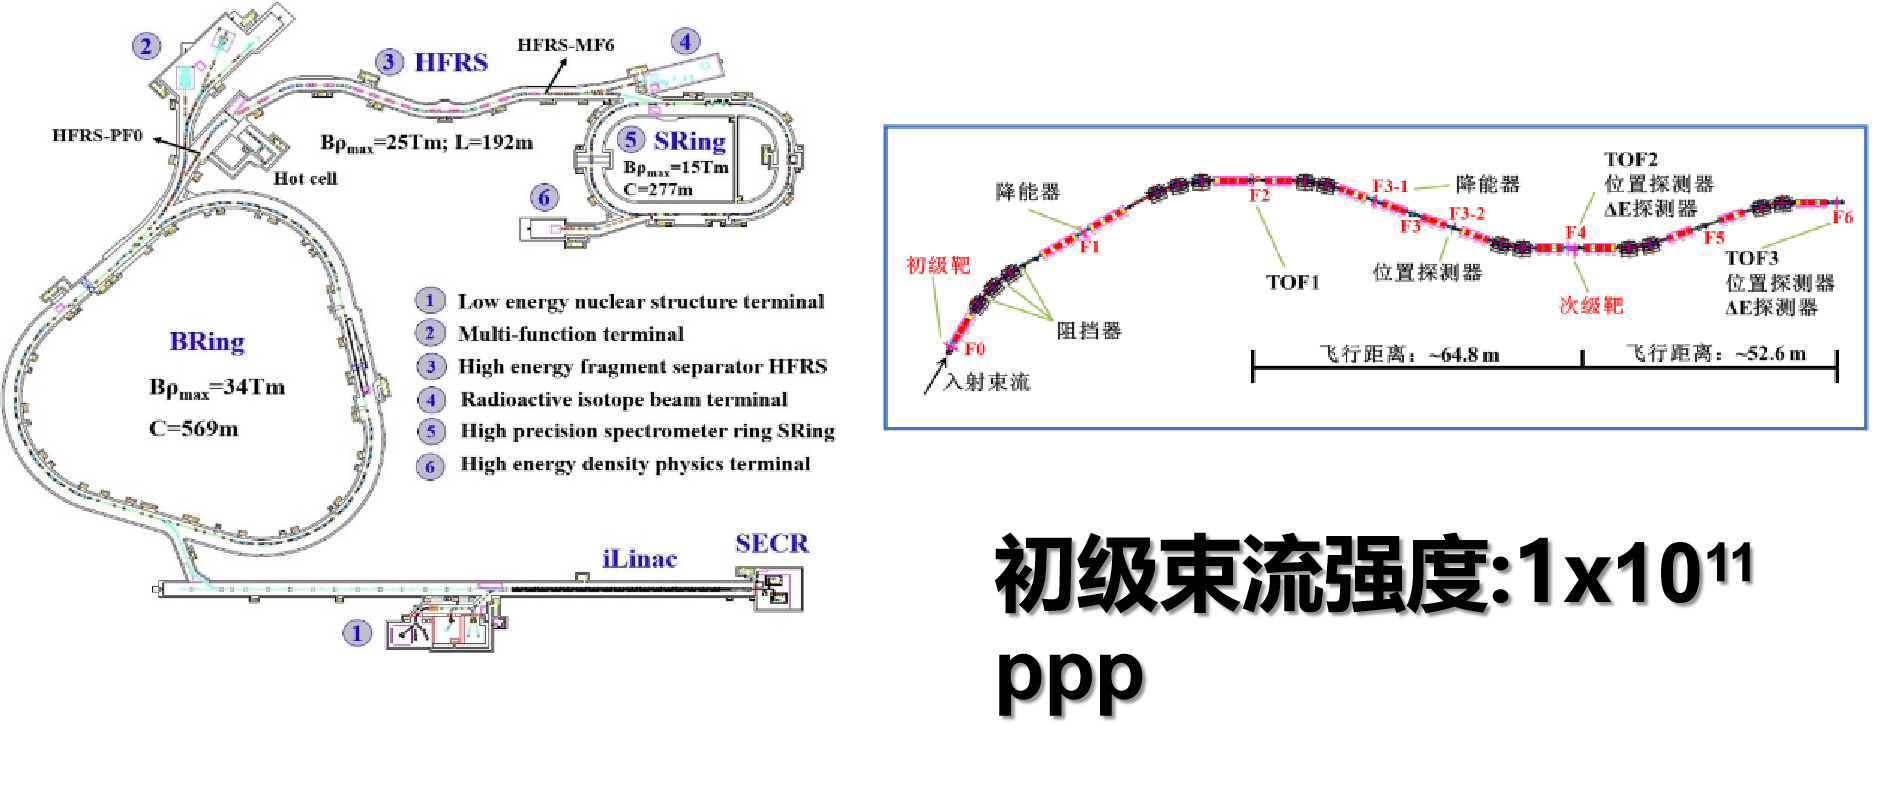
\includegraphics[width=0.8\textwidth]{pic/HIAF.png}
    \caption{HIAF束流装置示意图}
    \label{fig:setup0}
\end{figure}




%-----------------------------
\section{放射性束流能损探测器}
在核物理束流实验中，测量原子核经过探测器的能量沉积是鉴别原子核类型的关键一步。常见的能损探测器有气体探测器，半导体探测器以及闪烁体探测器。其中气体电离室是在放射性束流实验中最常见的能损探测器。因为半导体探测器受半导体器件的限制很难满足束流探测器需要的尺寸需求以及辐射耐受度，在长时间的束流照射下容易发生辐照损伤，探测性能下降。而闪烁体探测器通常有着很好的时间分辨率，但能量分辨率通常较差。因此，气体电离室凭借其抗辐照性能强、价格便宜、不受尺寸限制，广泛应用于放射性束流实验的能损探测。


气体电离室是指以气体作为探测介质的辐射探测器，利用辐射能量电离气体收集电子和重离子来测量能量。为了适用于放射性束流实验，提高电离室的能量分辨率和对高能离子的鉴别能力，在传统气体电离室的基础上进一步发展研制了多次取样电离室 (Multiple Sampling Ionization Chamber, MUSIC)，通过多次取样，显著提高气体电离室的能量分辨率，逐渐成为中高能粒子探测中最佳的能损测量探测器，并在多家实验室中得到了成功应用。成为了放射性束流能损实验中最广泛使用的能损探测器。探测器工作时，束流粒子入射至探测器灵敏体积内使工作气体电离产生电子和阳离子对；在电场的作用下，电子和阳离子分别向阳极与阴极漂移，漂移的同时在读出电极上产生感应电流信号。然而，当束流入射位置不同时，电子的漂移距离会有所不同，导致感应电流信号的持续时间也不同，使得信号幅度与束流入射位置相关。 MUSIC通过采用栅极隔离电场的方法解决了这个问题，只有电子穿过栅极才能在阳极感应出信号，此时栅极 - 阳极固定的间距可令感应电流信号的持续时间基本一致，从而消除了信号幅度与束流入射位置的相关性。另外，阳离子会向阴极漂移并被收集，它们不会穿过栅极。因此，栅极还能屏蔽阳离子对阳极信号的干扰。
\begin{figure}[htbp]
    \centering
    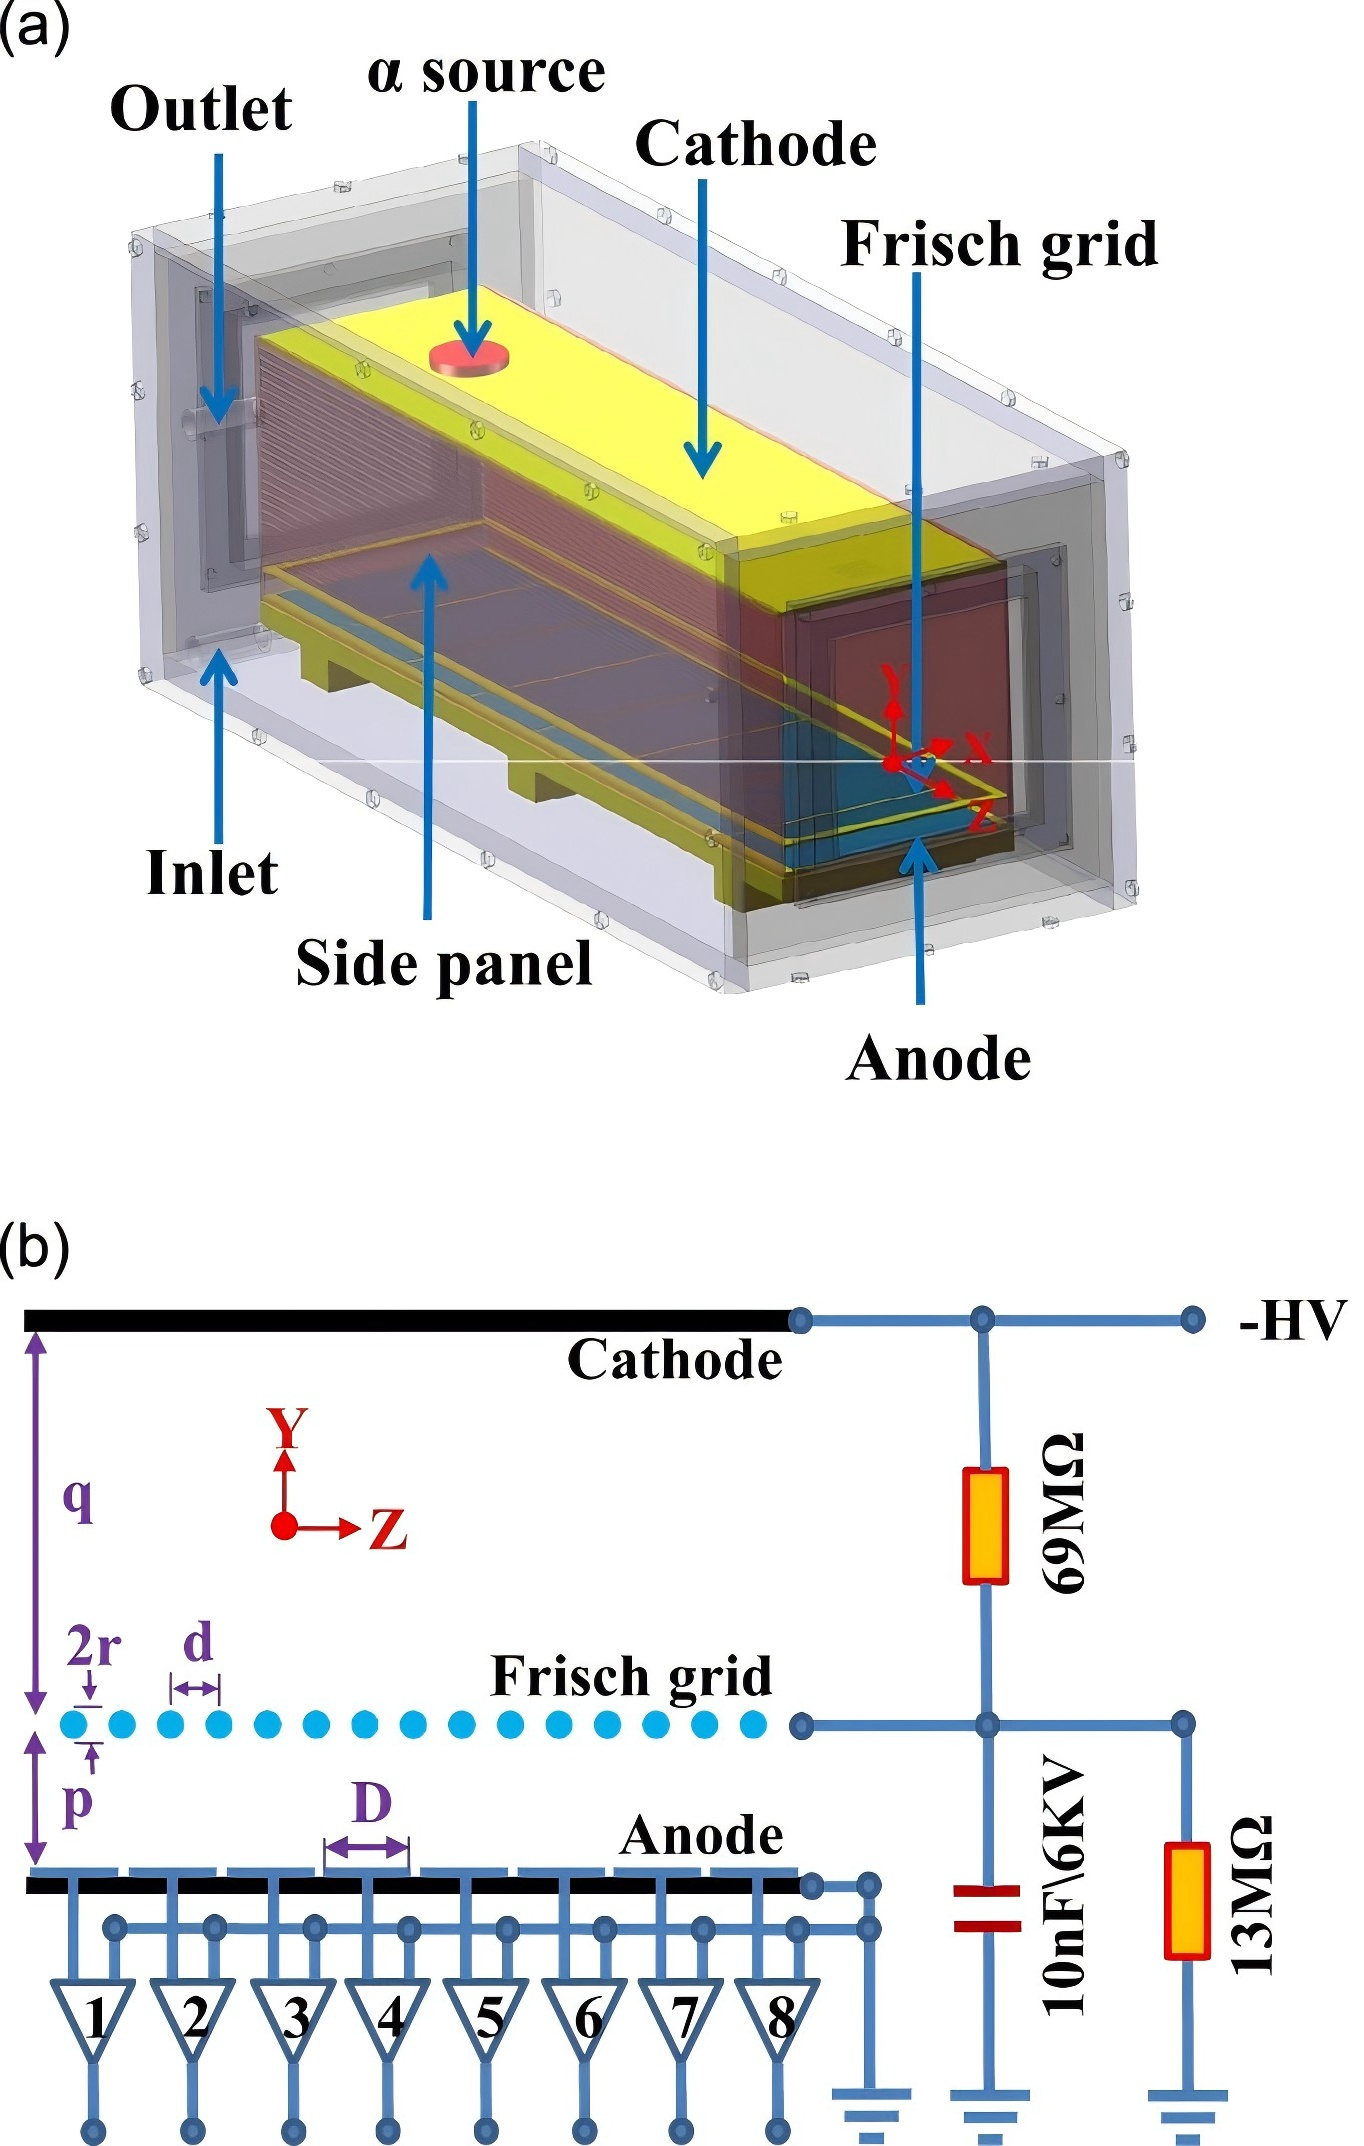
\includegraphics[width=0.45\textwidth]{pic/MUSIC.png}
    \caption{MUSIC探测器示意图}
    \label{fig:setup}
\end{figure}
MUSIC 探测器在放射性束流实验的广泛运用，主要得益于其良好的能量分辨和辐射耐受能力，以在 RIBLL2 束流线上开展的电荷改变截面测量实验为例，实验采用了两种架构的 MUSIC 进行能损测量，工作气体为 P10，腔体电极与水平方向呈 \(45^\circ\) 夹角从而对反应前和反应后的重离子进行鉴别。根据能损测量区分原子电荷的分辨率均达到了 0.2 以下，很好地满足了实验需求。

然而，MUSIC 在束流探测中存在一个不可忽略的问题，即由于栅极的存在，屏蔽了电子漂移时的感应信号，因为电子和正离子的产生和漂移都需要不可忽视的时间，从而在结构上给探测器带来了不可避免的死时间，大小在 \(10^{-6} \, \text{s}\) 量级，这是影响 MUSIC 时间分辨的一个重要因素。此外，为了提高信噪比，电离室还包含了低噪声，高增益，长衰减时间的前放，以及进行成形滤波的主放，导致信号出现较长的下降沿和成形时间，大概在 \(10 \, \mu\text{s}\) 左右，这也会影响电离室的时间分辨。当计数率升高时，会发生堆积（pile - up）事件，影响事件统计。在一般的束流实验中，MUSIC 的有效计数率通常在 \(10^5 \, \text{cps}\) 以下，否则堆积事件就会占到 40\% 以上，严重影响了束流的利用效率和实验的统计精度。
\begin{figure}[htbp]
    \centering
    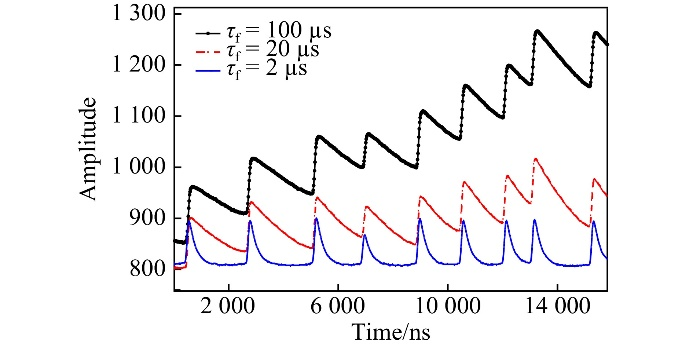
\includegraphics[width=0.45\textwidth]{pic/pileup事件.png}
    \caption{堆积事件信号示意图}
    \label{fig:setup}
\end{figure}

为了提高放射性束流能损测量的计数率，国内外各个实验组都在寻求进行改进。
针对 MUSIC 存在的死时间的问题，采取了更换工作气体以加快电子漂移速度[22],取消
栅极或者优化 MUSIC 电极结构等方法德国GSI[14] 将 MUSIC的工作气体由P10替换成电子漂移速度更快的CF4以减少探测器自身的死时间，并通过优化电荷灵敏前放与主放的成形时间，将计数率提高至200 kHz。日本 RIKEN[17]将 MUSIC的电极改为导电的薄膜平面，并使电极与束流成一定倾斜角，由于不带栅极,可使电离电子一开始漂移就在阳极上产生感应信号，从而消除探测器自身的死时间，再利用双极成形主放消除阳离子的影响，可以在将计数率提高至1 MHz时保证0.3以下的ΔZ分辨。

针对HIAF中的HFRS线，中国科学院近代物理研究所的研究团队提出了一种高计数率的能损探测器方案[13]。HFRS束流线具有极高的流强（初级束流强度为$1x10^{11}$ ppp），对能损探测器提出了非常高的计数率要求。研究团队通过优化探测器结构和读出方法，提高了探测器的响应速度，并采用快速电荷灵敏前放来初步放大信号，直接采样脉冲波形，并使用数字算法处理，以适应高计数率下的信号处理。这种利用波形数字化技术直接对前放的输出波形进行采样的方法，放弃使用主放，其优势有：数字化后 的信号不再受后级电路噪声干扰；波形数字化技术支持自触发方式获取波形，可以消除由于ADC门宽带来的死时间；在采集到了波形信息后，即使发生了堆积，还可以利用波形信息发展算法进行堆积修正。

\section{新一代半导体探测器}
半导体探测器是一种利用辐射产生的电子-空穴对来测量能量的探测器，具有高能量分辨率和快速响应的特点。传统的半导体探测器主要由硅，锗等材料制成，相较于气体探测器，具有较高的能量分辨率，并且，因其载流子更快的漂移速度，其时间分辨通常能达到ns量级。然而，此类探测器受制作工艺的限制，尺寸较小，且PN结在高能带电离子束流的照射下容易发生辐照损伤，导致性能下降，因此在针对放射性束流能损测量中的应用受限[6]。
如上节所述，第一代传统半导体探测器因为其易受辐照损伤的性质，不适用于高能带电离子束流探测[6]，而由化学气相沉积得到的金刚石等耐辐照能力较强的探测器，因其制作工艺往往只有大小只有几个微米，难以满足大型束流的测量任务，近些年来，随着半导体工业的不断发展，以SiC为代表的第三代半导体探测器凭借其耐辐照能力强，能带间隙宽的特点，逐渐也成为了离子束流线上常见的能损探测器。

\begin{figure}[htbp]
    \centering
    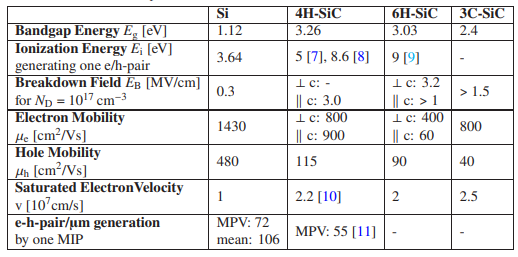
\includegraphics[width=0.45\textwidth]{pic/SIC性能对比.png}
    \caption{Si与SiC半导体探测器性能对比}
    \label{fig:setup}
\end{figure}

从表中可以看到，与硅相比，碳化硅的电离能、带隙和饱和电子速度更高。碳化硅的电荷迁移率低于硅。然而，由于高击穿电场和高漂移速度的结合，在碳化硅中产生的信号比在硅中产生的信号更快。第三代半导体探测器在束流检测方面最突出的应用是在放疗束流监控领域[22], 在离子癌症治疗中，高强度离子束通过利用布拉格峰来治疗肿瘤。典型的离子治疗使用的粒子速率高达 1010离子/秒进行治疗。当将这些束线用于粒子物理实验或作为测试束环境时，这样的强度通常过高。碳化硅 (SiC) 是这种应用的理想探测器材料，因为它结合了潜在的高辐射硬度和高热导率以避免冷却。此外，其高电子饱和速度允许非常快速的信号以减轻堆积效应。奥地利离子癌症治疗中心MedAustron[22]利用宽强度范围（kHz-GHz）和不同能量（60-800 MeV）的质子束对Si探测器和SiC探测器进行了测试，发现在最高达到109cps强度的束流情况下，SiC探测器依旧能够保证稳定的探测效率[22]
。此外，Zhongming Zhang[23]等系统研究了金刚石、碳化硅（SiC）、氧化镓（Ga2O3）和氮化镓（GaN）等四种材料的束流检测能力，相较于传统硅基探测器，第三代半导体材料能够提供更高的灵敏度和更快的响应速度。这有助于更精确地捕捉到束流的变化情况，并且可以在更短时间内完成测量。除此之外，Dirust[25]等还开发了基于金刚石单晶的X射线束流检测器，通过金刚石单晶检测X射线光束的束流质量。

在MoniDiam项目中[29]，研发了针对离子放疗的碳或质子束提供具有高检测效率的大面积光束探测器，以100 MHz计数率进行时间和能量测量。使用带有铝盘形表面金属化的金刚石测量了20至90 ps的信号上升时间分辨率和7至9\%的能量分辨率。

\begin{figure}[htbp]
    \centering
    \begin{subfigure}[t]{0.48\textwidth}
        \centering
        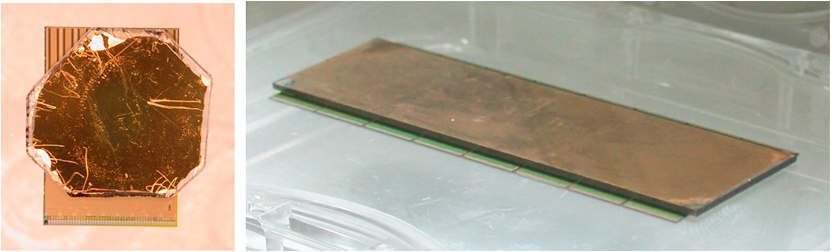
\includegraphics[width=\linewidth]{pic/金刚石.png}
        \caption{单晶金刚石及其封装}
        \label{fig:left}
    \end{subfigure}
    \hfill  % 或 \quad 控制间距
    \begin{subfigure}[t]{0.48\textwidth}
        \centering
        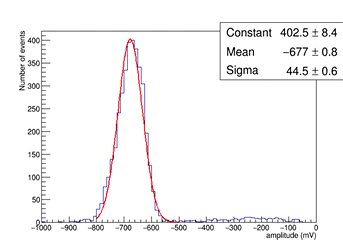
\includegraphics[width=\linewidth]{pic/金刚石分辨.png}
        \caption{单晶金刚石在95 MeV/u 碳束流下的能量分辨}
        \label{fig:right}
    \end{subfigure}
    \caption{单晶金刚石探测器}}
    \label{fig:both}
\end{figure}
可见，第三代半导体探测器已经广泛应用于各类束流检测及能损测量任务中，特别是在各类放疗治疗等医学物理项目中成果突出。然而，半导体探测器其固有的尺寸偏小，生长厚度不够等缺陷也限制了其对于重离子束流能损的监测，往往只能应用于如质子，中子等放疗使用的束线中或者作为位置分辨或时间探测器。此外，其昂贵的价格也限制了在大型束流实验中的应用。
\section{气氙探测器}
传统的闪烁体探测器虽然具有较好的时间分辨率，在束流实验中常用于时间标定；但其能量分辨率较差，难以满足放射性束流能损测量的需求。近年来，随着氙气探测器的不断发展，氙气探测器凭借其同时产生闪烁光和电离信号的能力，在核与粒子探测领域得到了广泛应用。氙气探测器具有高量子产额和较高的光子传输效率，使其成为放射性束流能损测量的有力工具。通过优化氙气探测器的设计和工作条件，可以实现更高的能量分辨率和更快的响应速度，为放射性束流实验提供更准确和可靠的能损测量结果。



RIKEN 最早在放射性束流能损探测领域引入气氙闪烁体探测器。研究团队开发了
一种气态氙闪烁体探测器作为新的 ΔE 探测器，预期具有好的辐射硬度和快速响应[26]。
新版本的探测器厚度与 RIBF 中当前标准 ΔE 探测的 MUSIC 相当，为 134mg/cm2
。在
RIBF 束流线上进行了探测器的性能测试，发现原子序数 Z 在 35 和 55 附近的均方根（rms）分
辨率分别约为0.2和0.3。此外，对于$^{238}$U束流，它具有良好的时间分辨率，为74.4(6)ps。
新开发的氙闪烁体探测器由 2 大气压和 9 厘米厚的氙气以及 125 微米厚的 φ40 毫米
Kapton 窗口组成，总厚度为 134 毫克/平方厘米，与 BigRIPS 中使用的离子室相当。由
于氙气发射的闪烁光子波长约为 175 纳米\cite{db}，因此使用了高透射率的特殊玻璃（Shin-Etsu 
Quartz SUPRASIL-P310C）作为窗口材料，以及在 175 纳米处具有 30\%高量子效率的特
殊 PMTs（Hamamatsu R6041-406）。为了实现高能量分辨率，探测器非常紧凑，长度仅
为 BigRIPS 中标准离子室的六分之一。但该探测器出现了一定程度的位置依赖, 即使
在考虑了位置校正后，探测器的信号仍显示出较大的位置依赖性。这种依赖性可能是
由于较大的立体角效应导致的。对于不同的束流位置，ΔE 分辨率会有所不同，远离中
心位置的束流会导致分辨率变差。而且，探测器不能保证性能的稳定性，在工作一个小
时以后，会存在明显的能量分辨降低等现象。
图12 在 Z = 35 设置下，87Br 的归一化电荷与从中心到光束命中位置的距离的平均
\begin{figure}[htbp]
    \centering
    \begin{subfigure}[t]{0.48\textwidth}
        \centering
        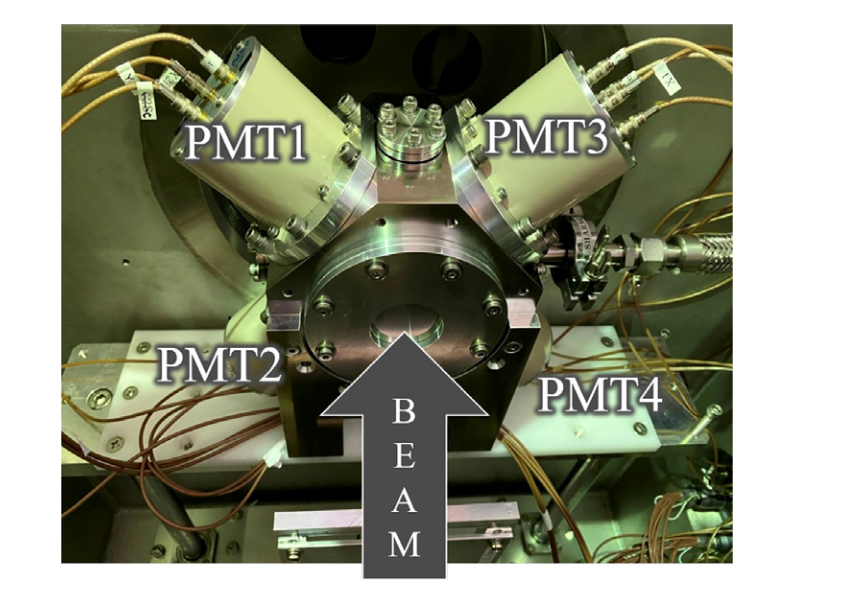
\includegraphics[width=\linewidth]{pic/RIKEN.png}
        \caption{RIKEN 氙闪烁体探测器}
        \label{fig:left}
    \end{subfigure}
    \hfill  % 或 \quad 控制间距
    \begin{subfigure}[t]{0.48\textwidth}
        \centering
        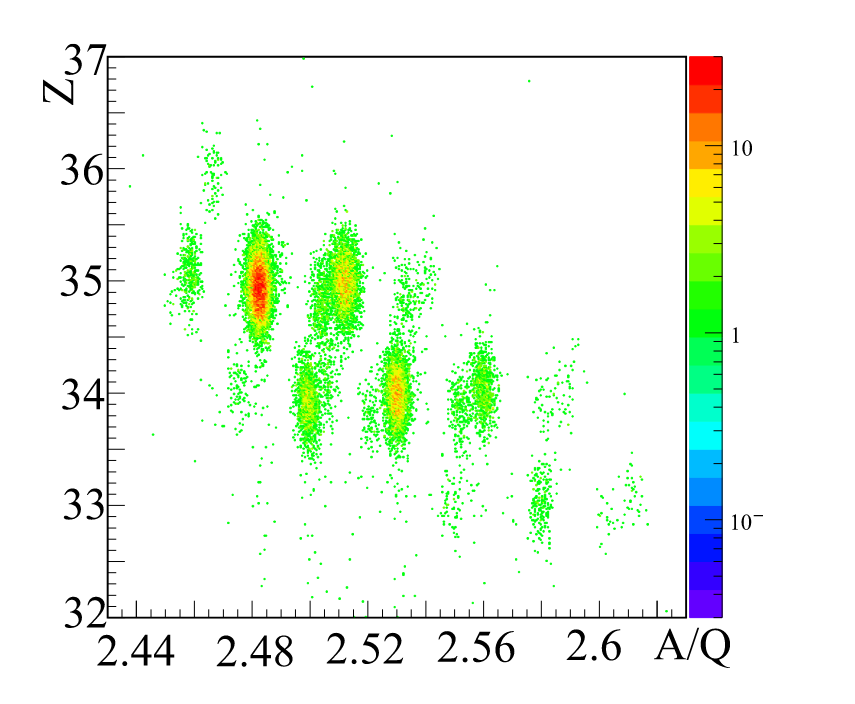
\includegraphics[width=\linewidth]{pic/粒子鉴别.png}
        \caption{气氙探测器能损粒子鉴别图}
        \label{fig:right}
    \end{subfigure}
    \caption{RIKEN 氙闪烁体探测器及性能测试结果}
    \label{fig:both}
\end{figure}

此外，美国 FRIB 束流也开发了一套能量损失光学闪烁系统（ELOSS）[27]。ELOSS
具有 30x60 cm²的矩形活跃区域，与 S800 焦平面的其他探测器（如跟踪探测器）相匹
配，有效厚度为 19 cm。该探测器由一个大型不锈钢室组成，内填充纯氙气，气体压力
可在 400 至 800 Torr 之间调节。探测器体积被分割成四个沿束流方向的扇区，每个扇
区宽 47 mm，周围均匀布置有光电倍增管（PMTs）以记录氙气的即时闪烁光。ELOSS
的完整光学读出由 120 个 Hamamatsu 一英寸 10 级 PMTs（型号 R8520-40615）组成，
这些 PMTs 在-110$^{°}C$ 至+50$^{°}C$ 的温度范围内工作，可承受高达 5 atm 的压力。PMTs 通
过正高压（HV）分压电路进行偏置，并通过定制的印刷电路板（PCB）进行机械支撑。
PMTs 的信号通过 Kapton 绝缘的微型同轴电缆传输。PMT 信号通过快速、高分辨率的
时间和幅度数字化器（Mesytec，型号 MDPP-32-QDC）进行处理。与 RIKEN 的气氙闪
烁体探测相比，FRIB 设计用于填充、调节和排空探测器体积。主要组件包括用于将氙
气注入系统的气体瓶架和压力调节器、在线去除杂质的净化系统、调节气体流动的控
制系统以及氙气回收/存储系统，保证了工作的稳定性。


\section{本文工作}
